\chapter[Il modello f-HDGM e l'algoritmo EM]{Introduzione all'analisi funzionale di dati spazio-tempo tramite il modello f-HDGM e cenni sull'algoritmo EM}

In questo primo capitolo, dopo aver presentato il concetto di analisi funzionale (\textit{Functional Data Analysis}, o \textit{FDA}), viene illustrato il modello spazio-temporale oggetto dell'estensione presentata in questo studio, ossia il \textit{Functional Hidden Dynamic Geostatistical Model} (o \textit{f-HDGM}). Infine, vengono fornite alcune nozioni per comprendere il funzionamento e, in primis, l'idea su cui si basa l'\textit{algoritmo EM}.

\section[Cenni sull'analisi funzionale dei dati]{Cenni sull'analisi funzionale dei dati}

\subsection[Differenza tra statistica inferenziale e analisi funzionale]{Differenza tra statistica inferenziale e analisi funzionale}
Fornito un campione di dati $D = (x_1, y_1), (x_2, y_2)\dots (x_N, y_N)$ e un modello $y = f(x, \boldsymbol{\theta}_0)$, l'obiettivo della statistica inferenziale è quello di stimare i parametri $\boldsymbol{\theta}_0$ andando a minimizzare una funzione di costo $J(\boldsymbol{\theta})$, ossia individuare la combinazione di valori stimati dei parametri $\boldsymbol{\hat{\theta}}_N$ tale che $\boldsymbol{\hat{\theta}}_N = \text{arg}\,\min\limits_{\boldsymbol{\theta}} J(\boldsymbol{\theta}, D)$. La funzione di costo cambia a seconda del modello da identificare e della tipologia di stima che viene utilizzata, per esempio OLS o MLE. Inoltre, non sempre è possibile risolvere il problema di minimo in forma chiusa\footnote{impiego di un'espressione matematica, esente da variabili libere, per calcolare il valore del parametro incognito. La ricerca iterativa dell'ottimo tramite un algoritmo non è necessaria.}; spesse volte è necessario ricorrere a tecniche di ottimizzazione numerica, in particolare quando la funzione $J(\boldsymbol{\theta})$ non è convessa. \par Nell'analisi funzionale, invece, l'oggetto della stima non è $\boldsymbol{\theta}$, ma la funzione $f$ continua. Le spline sono una delle classi di funzioni più utilizzate in FDA; la possibilità di regolare  la \textit{smoothness} rende loro facilmente generalizzabili.

\subsection[Basi di Fourier]{Basi di Fourier}
Le basi di Fourier sono una classe di spline che viene impiegata per descrivere segnali periodici. Il modello che il toolbox FDA per MATLAB~\cite{paper_FDA_toolbox} implementa è:
\[
	y(t) = \sqrt{2f}\cdot w(t)\\;
\]
\[
	w(t) = \frac{a_0}{\sqrt{2}} + \mathbf{a}_1\cdot \mathbf{k}_1(t)^\top +\dots + \mathbf{a}_i\cdot \mathbf{k}_i(t)^\top + \dots + \mathbf{a}_n\cdot \mathbf{k}_n(t)^\top;
\]
\[
	\mathbf{a}_i\in\mathbb{R}^{1\times2} =
	\begin{bmatrix}
		a_{i, \sin} & a_{i, \cos}
	\end{bmatrix};
\]
\[
	\mathbf{k}_i(t)\in\mathbb{R}^{1\times 2} =
	\begin{bmatrix}
		\sin\left(i\cdot\omega_0\cdot t\right) & \cos\left(i\cdot\omega_0\cdot t\right)
	\end{bmatrix}.
\]
$f$ è la frequenza, $n$ indica il numero di armoniche\footnote{il numero di basi è $n\cdot 2 + 1$.}, $\omega_0 = 2\pi\cdot f$ rappresenta la pulsazione dell'armonica fondamentale, mentre $a_0, a_1,\dots a_n$ sono i coefficienti combinatori. Oltre alla parte costante, ciascuna funzione seno e coseno costituisce una base. Una volta scelto il valore di $n$ a seconda del livello di complessità desiderato, l'obiettivo dell'analisi funzionale è quello di calcolare i coefficienti. Nelle figure \ref{esempi_Fourier} e \ref{esempio_Fourier_coef_non_unitari} sono riportati degli esempi sia di funzioni base sia di spline\footnote{combinazione lineare di basi di Fourier.}.

\begin{figure}[htp]
	\centering
	\subfigure[]{\label{}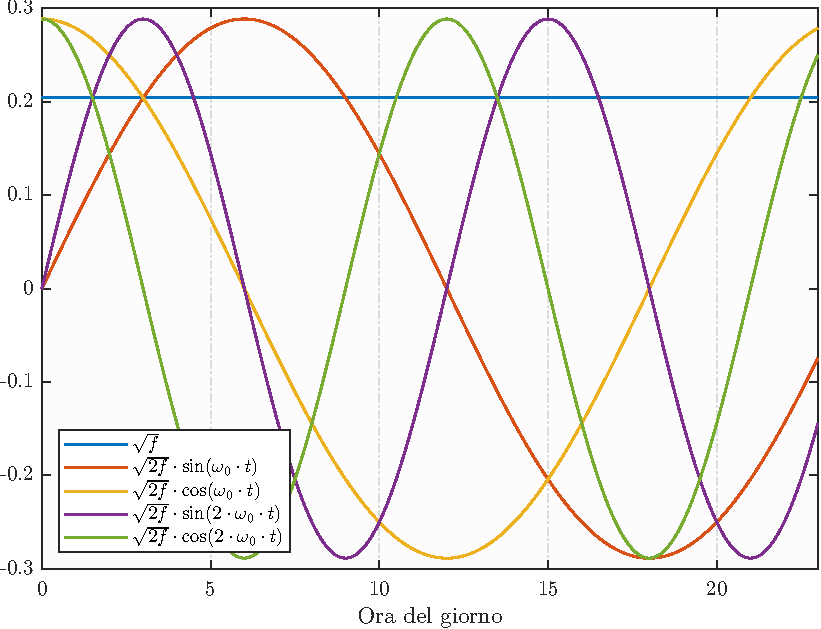
\includegraphics[height=158px]{Immagini/Modello base/Basi Fourier}}\quad
	\subfigure[]{\label{}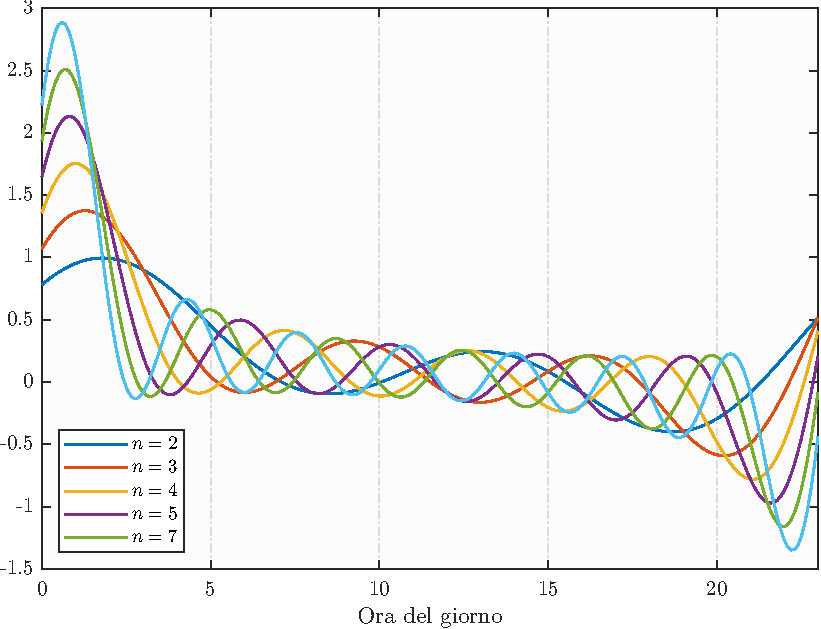
\includegraphics[height=158px]{Immagini/Modello base/Spline Fourier}}
	\caption[Confronto tra funzioni base con $n=2$ e tra diverse spline di Fourier]{confronto tra funzioni base con $n=2$ (a) e tra diverse spline di Fourier (b) i cui coefficienti combinatori sono unitari. Da notare come all'aumentare di $n$ la funzione risultante tenda al livello basso di un'onda quadra.}
	\label{esempi_Fourier}
\end{figure}
\begin{figure}[htp]
	\centering
	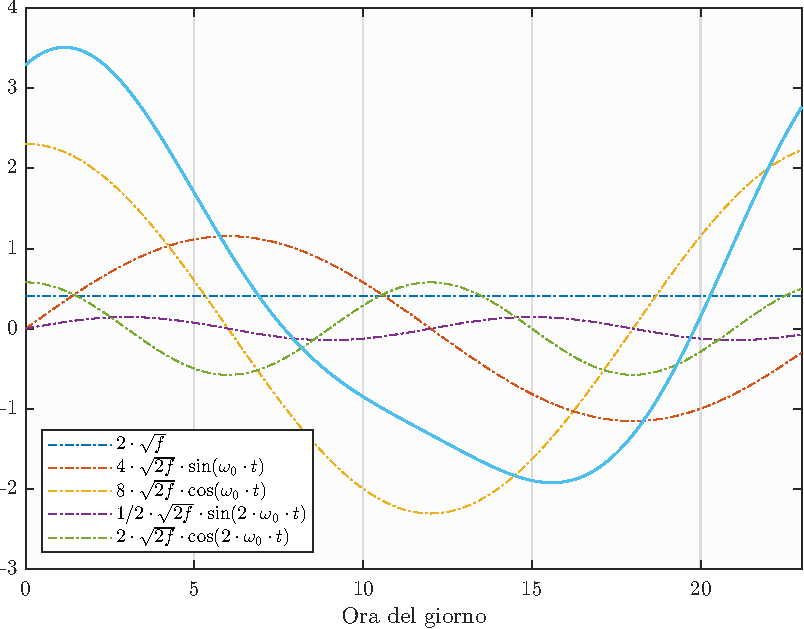
\includegraphics[height=180px]{Immagini/Modello base/Spline Fourier con coefficienti non unitari}
	\caption[Esempio di spline di Fourier con $n=2$ i cui coefficienti combinatori sono diversi da \num{1}]{esempio di spline di Fourier (in azzurro) con $n=2$ i cui coefficienti combinatori sono diversi da \num{1}. Nello specifico: $a_0 = 2$, $a_{1,\sin} = 4$, $a_{1,\cos} = 8$, $a_{2,\sin} = 1/2$ e $a_{2,\cos} = 2$.}
	\label{esempio_Fourier_coef_non_unitari}
\end{figure}

\subsection[Analisi funzionale e dati spazio-tempo]{Analisi funzionale e dati spazio-tempo}
Si ipotizzi di avere a disposizione i dati di temperatura acquisiti da due sensori collocati in due punti distinti di una stanza, ossia $T(\mathbf{s}_1, t)$ e $T(\mathbf{s}_2, t)$. La correlazione spaziale esistente tra punti, in aggiunta all'autocorrelazione temporale, può essere impiegata per prevedere la temperatura in una terza posizione $\mathbf{s}_3$ all'istante di tempo $t_0$. Per eseguire questa operazione utilizzando un modello non funzionale, tuttavia, è necessario conoscere sia $T(\mathbf{s}_1, t_0)$ sia $T(\mathbf{s}_2, t_0)$, una condizione che potrebbe non verificarsi sempre nel caso in cui i due sensori siano \textit{asincroni}. A questo punto sarebbe necessario ricorrere a una delle tecniche di interpolazione note in letteratura per stimare i dati mancanti, strategie che inevitabilmente introducono del rumore nel modello. \par L'indipendenza dalla sincronia e dalla continuità delle serie storiche rendono i modelli funzionali particolarmente adatti a risolvere situazioni di questa natura; una volta stimata la funzione $f$, infatti, è possibile utilizzarla per effettuare predizioni in qualsiasi punto e in qualsiasi istante.

\section[Il modello f-HDGM]{Il modello f-HDGM}
Il Functional Hidden Dynamic Geostatistical Model è stato illustrato in un articolo scientifico pubblicato sul Journal of Statistical Software nel settembre del \num{2021}, un paper finalizzato a presentare, oltre al modello, anche D-STEM v2, un software il cui scopo è stimare tramite l'algoritmo EM una serie di modelli spazio-temporali~\cite{paper_f_HDGM}.

\subsection[Equazioni del modello]{Equazioni del modello}
\label{equazioni_modello_base}
Sia $\mathbf{s} = (s_{lon}, s_{lat})^\top$ un generico punto spaziale sulla sfera terrestre $\mathbb{S}^2$ e $t\in\mathbb{N}$ un indice temporale discreto. Si assume che la funzione di interesse $f(\mathbf{s}, l, t)$, con dominio $\mathcal{L}=[l_1, l_q]\subset\mathbb{R}$, possa essere osservata in ogni $(\mathbf{s}, t)$ ed $l\in \mathcal{L}$ attraverso delle misurazioni rumorose $y(\mathbf{s}, l, t)$ che seguono il seguente modello matematico:
\begin{equation}
	y(\mathbf{s}, l, t) = f(\mathbf{s}, l, t) + \epsilon(l);
	\label{eq_rumore_uscita}
\end{equation}
\begin{equation}
	f(\mathbf{s}, l, t) = \mathbf{x}(\mathbf{s}, l, t)^\top\cdot\boldsymbol{\beta}(l) + \Phi(l)^\top\cdot\mathbf{z}(\mathbf{s}, t);
	\label{eq_comp_det}
\end{equation}
\begin{equation}
	\mathbf{z}(\mathbf{s}, t) = G\cdot \mathbf{z}(\mathbf{s}, t-1) + \boldsymbol{\eta}(\mathbf{s}, t).
	\label{eq_comp_lat}
\end{equation}
Prima di entrare in medias res, è bene introdurre la nomenclatura che successivamente verrà utilizzata per definire nel modello le dimensioni degli oggetti matriciali e vettoriali:
\begin{itemize}
	\item $n$ indica il numero di posizioni spaziali (o punti di misura) $\mathbf{s}\in\mathbb{R}^2$ prese in esame;
	\item $q$ rappresenta la dimensione del dominio (funzionale) $\mathcal{L}$ rappresentante l'alta frequenza. Se, per esempio, tramite l'indice discreto $h$ ci si vuole riferire all'ora del giorno, allora $q=24$ (da $0$ a $23$ con risoluzione $1$);
	\item $T$ indica il numero di campioni in bassa frequenza, ad esempio i giorni. In assenza di dati mancanti, il singolo campione è costituito da $n\cdot q = N$ osservazioni (per ognuna delle $n$ posizioni spaziali sono note tutte le $q$ rilevazioni della variabile $y$, una per ogni ora del giorno);
	\item $b$ rappresenta il numero di variabili esplicative, ovvero $|\boldsymbol{\beta}(l)| = b$;
	\item infine, $n_\epsilon$, $n_\beta$ ed $n_z$ indicano il numero di funzioni base utilizzate per modellare rispettivamente $\sigma_\epsilon (l)$, ogni $\beta(l)$ e $\Phi(l)$ per $\mathbf{z}(\mathbf{s}, t)$.
\end{itemize}
Da sottolineare che attualmente non esiste una versione multi-variata\footnote{$\mathbf{y}(\mathbf{s}, l, t)\in\mathbb{R}^{p\times 1}$, con $p>1$.} dell'f-HDGM.

\subsection[Rumore sull'uscita]{Rumore sull'uscita}
Nell'equazione \ref{eq_rumore_uscita}, $\epsilon (l)\in\mathbb{R}$ è una variabile causale con distribuzione gaussiana avente media nulla ($\mu_\epsilon = 0$), indipendente sia nello spazio sia nel tempo. La sua varianza $\sigma_\epsilon(l)$ è \textit{eteroschedastica}\footnote{dato un campione di variabili casuali, al suo interno esistono delle sotto-popolazioni che hanno diverse varianze.} nel dominio $\mathcal{L}$; essa è modellata nel modo seguente:
\[
	\log(\sigma_\epsilon(l)) = \Phi(l)^\top\cdot\mathbf{c}_\epsilon.
\]
$\Phi(l)\in\mathbb{R}^{n_\epsilon\times 1}$ sono le $n_\epsilon$ funzioni base valutate in $l$, mentre $\mathbf{c}_\epsilon\in\mathbb{R}^{n_\epsilon\times 1}$ i rispettivi coefficienti combinatori da stimare. \par La finalità della modellazione funzionale della varianza consiste nell'adattare il livello di incertezza in base a vari fattori, come ad esempio l'orario del giorno. Ciò è dovuto al fatto che il numero di osservazioni disponibili per ciascuna delle $q$ fasce orarie non rimane costante.

\subsection[Componente deterministica]{Componente deterministica}
Nell'equazione \ref{eq_comp_det}, $\mathbf{x}(\mathbf{s}, l, t)\in\mathbb{R}^{b\times 1}$ è un vettore di variabili esplicative, i cui coefficienti moltiplicativi $\boldsymbol{\beta}(l) = (\beta_1(l),\dots,\beta_b(l))^\top$ sono così espressi:
\[
	\beta_j(l) = \Phi(l)^\top\cdot\mathbf{c}_{\beta, j}.
\]
$\Phi(l)\in\mathbb{R}^{n_\beta\times 1}$ sono le $n_\beta$ basi valutate in $l$, mentre $\mathbf{c}_{\beta, j}\in\mathbb{R}^{n_\beta\times 1}$ i rispettivi coefficienti della variabile $j$ da stimare. Piuttosto che considerare un effetto globale tempo-invariante, l'utilizzo delle spline consente di far variare il peso attribuito a ciascun regressore nel dominio $\mathcal{L}$. \par Si ipotizzi, per esempio, di voler descrivere la concentrazione di anidride carbonica $y_{CO_2}(\mathbf{s}, l, t)$ rilevata nel tempo da una stazione di misura in funzione dell'umidità relativa $x_{rel}(\mathbf{s}, l, t)$. Probabilmente il loro legame cambia a seconda dell'ora del giorno, un effetto che, inoltre, potrebbe mutare da un giorno all'altro; infatti, non è detto che l'umidità relativa descriva la concentrazione dell'inquinante in oggetto sempre nello stesso modo, sia in estate che in inverno, in tutti i punti spaziali. Per modellare questa variabilità spazio-temporale subentrano i coefficienti $z(\mathbf{s}, t)$, ovvero la componente latente.

\subsection[Componente latente]{Componente latente}
Nell'equazione \ref{eq_comp_lat}, $z(\mathbf{s}, t)\in \mathbb{R}^{n_z\times 1}$ è una variabile latente spazio-temporale avente una dinamica markoviana descritta da $G\in\mathbb{R}^{n_z\times n_z}$, una matrice di transizione diagonale\footnote{si assume che la cross-covarianza sia nulla.}. Il vettore delle innovazioni $\boldsymbol{\eta}(\mathbf{s}, t)\in\mathbb{R}^{n_z\times 1}$ si ottiene da un processo gaussiano multi-variato, indipendente nel tempo ma correlato nello spazio mediante la seguente matrice di covarianza funzionale:
\[
	\Gamma(\mathbf{s}, \mathbf{s}';\boldsymbol{\theta})=\text{diag}(v_1\cdot\rho(\mathbf{s}, \mathbf{s}';\theta_1),\dots,v_{n_z}\cdot\rho(\mathbf{s}, \mathbf{s}';\theta_{n_z})).
\]
$\mathbf{v}\in\mathbb{R}^{n_z\times 1}$ è un vettore di varianze, mentre $\rho(\mathbf{s}, \mathbf{s}'; \theta_j)$ è una funzione di correlazione spaziale idonea per i punti spaziali $\mathbf{s}, \mathbf{s}'\in\mathbb{S}^2$ parametrizzata tramite $\theta_j$, $\boldsymbol{\theta}\in\mathbb{R}^{n_z\times 1}$ (ogni variabile latente ha la sua parametrizzazione). Per concludere:
\begin{itemize}
	\item il vettore $\mathbf{v}$ è la diagonale della matrice diagonale $V\in\mathbb{R}^{n_z\times n_z}$. Infatti, si assume che le $n_z$ variabili latenti siano tra di loro indipendenti (nullità dei termini extra-diagonale), ossia $\eta_1(\mathbf{s}, t)\ \bot\ \eta_2(\mathbf{s}, t)\ \bot\dots\bot \ \eta_{n_z}(\mathbf{s}, t)$;
	\item un esempio di funzione di correlazione spaziale $\rho$ è quella esponenziale, ovvero $\rho(\mathbf{s}, \mathbf{s}'; \theta_j) = e^{-\frac{\lvert\mathbf{s} - \mathbf{s}'\lvert}{\theta_j}}$.
\end{itemize}

\paragraph{Simulazione di un processo spaziale gaussiano}
In un contesto spaziale, è possibile interpretare un processo gaussiano come un insieme (o campo) di variabili casuali che mostrano correlazioni spaziali tra di loro. Si ipotizzi di trovarsi in un piano cartesiano regolare di dimensioni $100\times100$ ($n=10^4$) e che $n_z =2$, il quale corrisponde al numero di processi (tra di loro indipendenti se $V$ è diagonale). Il processo può essere modellato tramite la normale multi-variata:
\[
	\begin{bmatrix}
		\eta_1 \\
		\eta_2 \\
	\end{bmatrix}\backsim \mathcal{N}_N\left\{\boldsymbol{\mu}=[\mathbf{0}]_{N\times 1}, \Gamma = 
	\begin{bmatrix}
		v_1\cdot I_{n}\cdot [e^{-\frac{D}{\theta_1}}]_{n\times n} & [\mathbf{0}]_{n\times n} \\
		[\mathbf{0}]_{n\times n} & v_2\cdot I_{n}\cdot [e^{-\frac{D}{\theta_2}}]_{n\times n} \\
	\end{bmatrix}_{N\times N}
	\right\}.
\]
$D\in\mathbb{R}^{n\times n}$ è la matrice delle distanze, $N=n_z\cdot n = 2\cdot 10^4$ rappresenta il numero totale di variabili aleatorie e $I_n\in\mathbb{R}^{n\times n}$ è una matrice identità di ordine $n$.
\par I coefficienti $\boldsymbol{\theta} = (\theta_1,\theta_2)^\top$ descrivono la velocità con la quale, fissato $\mathbf{s}$, le v.c. collocate nelle altre posizioni spaziali $\mathbf{s}'$ tendono ad assumere un valore diverso da quello assunto dal processo gaussiano in $\mathbf{s}$ all'aumentare della distanza $|\mathbf{s} - \mathbf{s}'|$. Nella figura \ref{sim_proc_gaussiano} è possibile notare come la variabilità del processo tenda a diminuire all'aumentare di $\theta$ a causa della maggiore correlazione esistente tra punti vicini, un comportamento osservabile anche nei valori assunti dalla densità di probabilità congiunta della normale bi-variata ottenuta scegliendo due variabili causali.

\begin{figure}[h!]
	\centering
	\subfigure[]{\label{}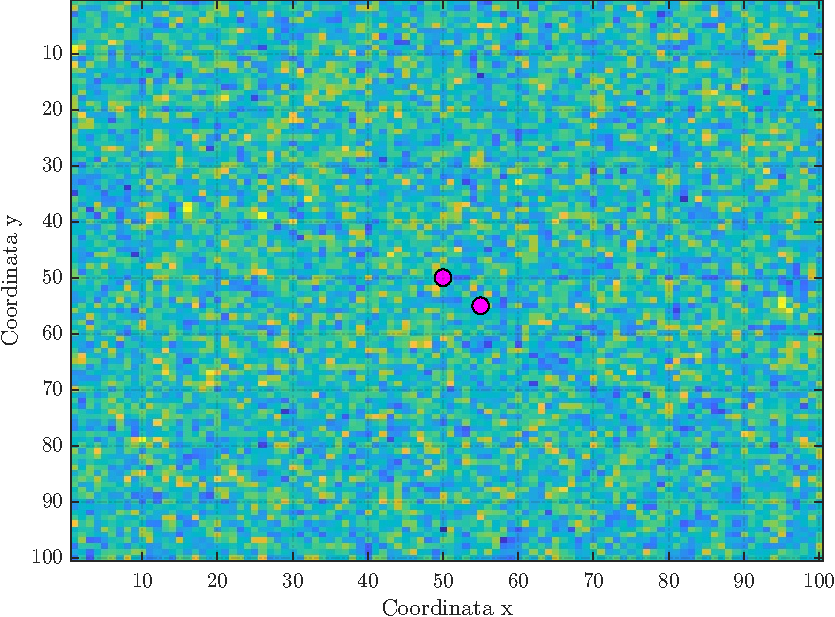
\includegraphics[height=152px]{Immagini/Modello base/Sim. proc. gaussiano, theta = 0.5}}\quad
	\subfigure[]{\label{}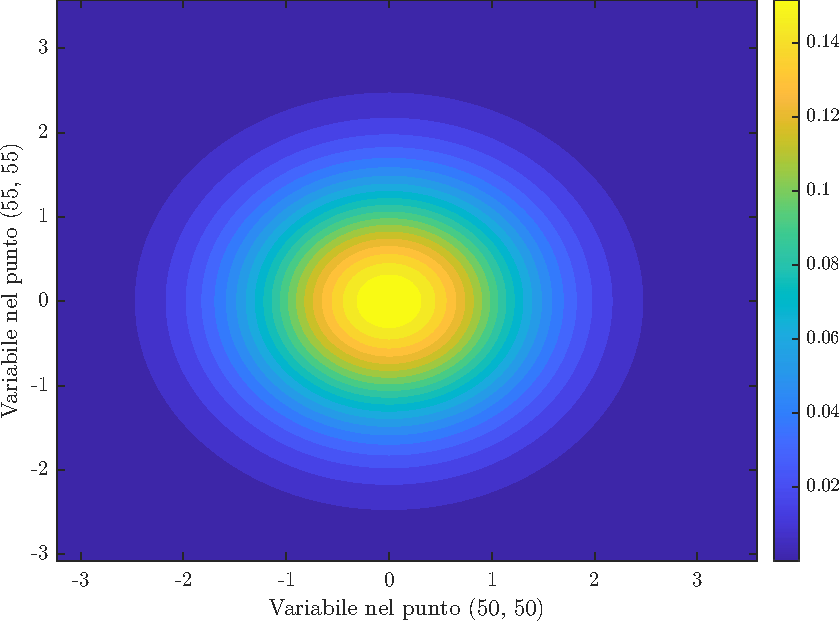
\includegraphics[height=152px]{Immagini/Modello base/Sim. var. casuali, theta = 0.5}}\quad
	\subfigure[]{\label{}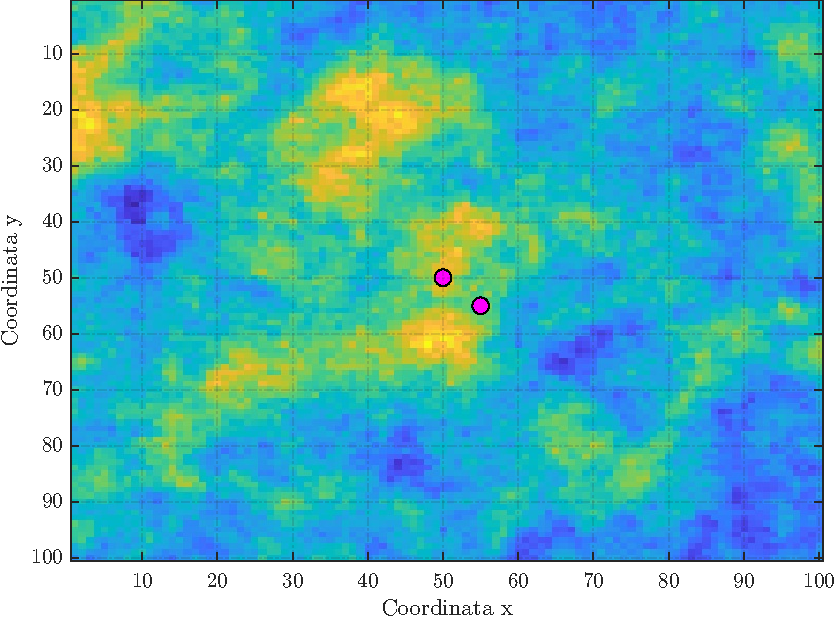
\includegraphics[height=152px]{Immagini/Modello base/Sim. proc. gaussiano, theta = 10}}\quad
	\subfigure[]{\label{}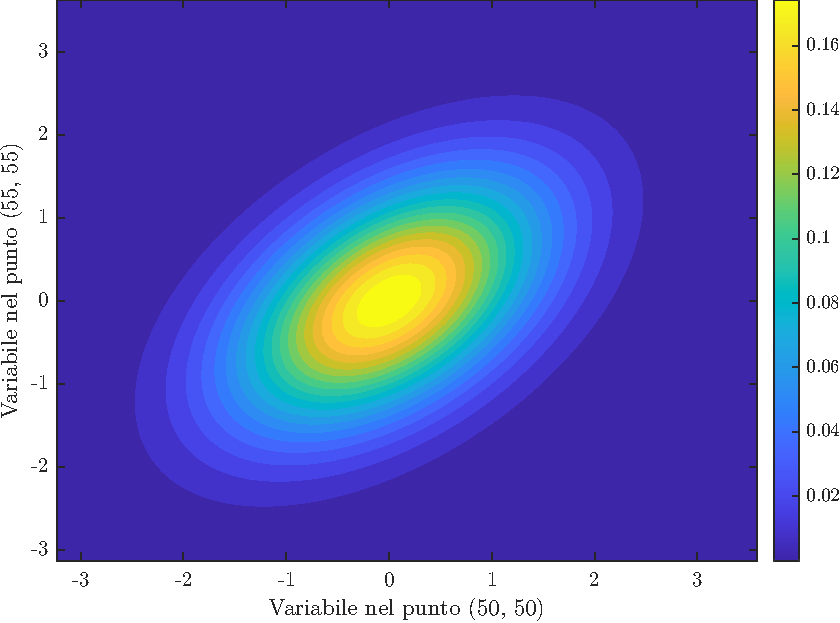
\includegraphics[height=152px]{Immagini/Modello base/Sim. var. casuali, theta = 10}}\quad
	\subfigure[]{\label{}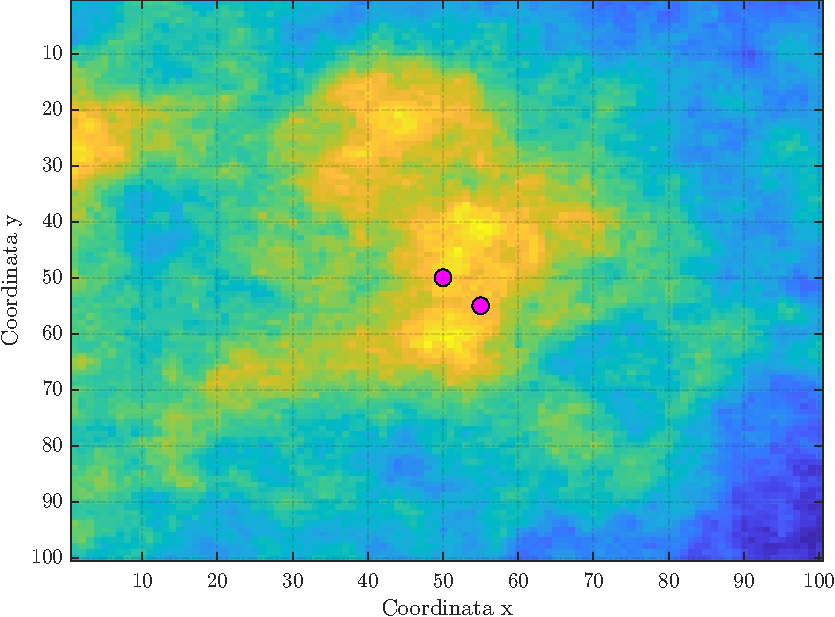
\includegraphics[height=152px]{Immagini/Modello base/Sim. proc. gaussiano, theta = 100}}\quad
	\subfigure[]{\label{}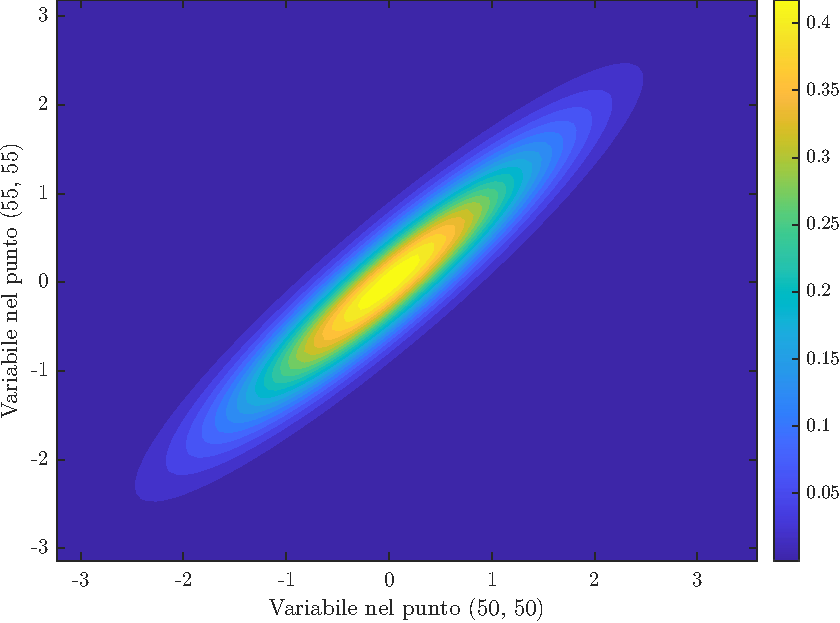
\includegraphics[height=152px]{Immagini/Modello base/Sim. var. casuali, theta = 100}}
	\caption[Simulazione di un processo spaziale gaussiano su un piano cartesiano al variare di $\theta$]{simulazione di un processo spaziale gaussiano su un piano cartesiano regolare e rispettiva densità di probabilità congiunta della normale bi-variata riferita ai punti $(50, 50)$ e $(55, 55)$ con $\theta=0.5$ (a, b), \num{10} (c, d) e \num{100} (e, f).}
	\label{sim_proc_gaussiano}
\end{figure}

\subsection[Parametri da stimare]{Parametri da stimare}
In conclusione, viene riportato il vettore $\boldsymbol{\psi}\in\mathbb{R}^{(n_\epsilon + n_\beta\cdot b + 3\cdot n_z)\times 1}$ contenente i parametri da stimare:
\begin{equation}
	\boldsymbol{\psi} = (\mathbf{c}_\epsilon^\top, \mathbf{c}_\beta^\top, \mathbf{g}^\top, \mathbf{v}^\top, \boldsymbol{\theta}^\top)^\top.
\end{equation}
Alcuni di essi possono essere calcolati in forma chiusa, altri richiedono l'ottimizzazione numerica.
\par Inoltre, è necessario ricostruire la componente latente, operazione complessa che può essere eseguita integrando il filtro di Kalman (e smoother) nel passo E dell'algoritmo EM.

\section[Cenni sull'algoritmo EM]{Cenni sull'algoritmo EM}
L'algoritmo EM (Expectation-Maximization) è una tecnica di ottimizzazione iterativa per determinare la stima a massima verosimiglianza (Maximum Likelihood Estimate, o MLE) \textbf{in presenza di dati mancanti o nascosti (variabili latenti)}. Nella stima ML si desidera determinare i parametri del modello per i quali i dati osservati risultano essere i più verosimili~\cite{paper_EM_algorithm}. \par Ogni iterazione dell'algoritmo EM consiste in due passi:
\begin{itemize}
	\item \textbf{passo E}: a partire dalla stima corrente dei parametri $\boldsymbol{\theta}_n$ e dai dati disponibili $\mathbf{x}$, quelli mancanti e/o nascosti vengono prima stimati e poi impiegati per determinare l'\textit{aspettativa condizionale} $Q(\boldsymbol{\theta},\boldsymbol{\theta}_n)$, una semplificazione della stima corrente della funzione di verosimiglianza $l(\boldsymbol{\theta}|\boldsymbol{\theta}_n)$;
	\item \textbf{passo M}: $Q(\boldsymbol{\theta},\boldsymbol{\theta}_n)$ viene ottimizzata per determinare $\boldsymbol{\theta}_{n+1}$, assumendo che i dati mancanti siano noti. Le stime di questi, ottenute precedentemente nel passo E, sono utilizzate al posto dei dati mancanti effettivi.
\end{itemize}
La convergenza dell'algoritmo è garantita dall'aumento della verosimiglianza a ogni iterazione.

\subsection{Derivazione del passo E}
Sia $\mathbf{x}$ un vettore di dati aleatori appartenenti a una famiglia di modelli parametrizzata. Si desidera trovare il valore delle incognite $\boldsymbol{\theta}$ tale che la verosimiglianza $L(\boldsymbol{\theta})=P(\mathbf{x} | \boldsymbol{\theta})$ sia massima. L'algoritmo EM garantisce che $L(\boldsymbol{\theta}) > L(\boldsymbol{\theta}_n)$; applicando il logaritmo naturale\footnote{semplificazione che spesse volte viene adottata per trasformare il prodotto di densità di probabilità che caratterizza $L$ (assumendo l'indipendenza tra i campioni) in una somma.} si ottiene:
\begin{equation}
	\ln(P(\mathbf{x}|\boldsymbol{\theta}) - P(\mathbf{x}|\boldsymbol{\theta}_n)) > 0.
	\label{eq_dis_verosimiglianza}
\end{equation}
Tale risultato deriva dal fatto che $L(\boldsymbol{\theta})$ si può dimostrare essere strettamente positiva. Tuttavia, i dati osservati $\mathbf{x}$ non dipendono soltanto dai parametri da stimare, ma anche dai valori assunti dalle componenti latenti $\mathbf{z}$ (da ricostruire utilizzando il filtro di Kalman). Infatti, la probabilità totale $P(\mathbf{x}|\boldsymbol{\theta})$ può essere riscritta in termini di $\mathbf{z}$ come:
\[
	P(\mathbf{x}|\boldsymbol{\theta}) = \sum_{\mathbf{z}}^{}P(\mathbf{x}|\boldsymbol{\theta}, \mathbf{z})\cdot P(\mathbf{z}|\boldsymbol{\theta}).
\]
Di conseguenza, l'equazione \ref{eq_dis_verosimiglianza} diventa:
\begin{equation}
	L(\boldsymbol{\theta}) - L(\boldsymbol{\theta}_n) = \ln\sum_{\mathbf{z}}^{} P(\mathbf{x}|\boldsymbol{\theta}, \mathbf{z})\cdot P(\mathbf{z}|\boldsymbol{\theta}) - \ln P(\mathbf{x}|\boldsymbol{\theta}_n).
	\label{eq_dis_verosimiglianza_completa}
\end{equation}
A partire dall'introduzione del termine \textcolor{orange}{$P(\mathbf{z}|\mathbf{x},\boldsymbol{\theta}_n)$} nell'equazione \ref{eq_dis_verosimiglianza_completa}, è possibile eseguire la seguente derivazione:
\begin{equation}
	\begin{split}
		L(\boldsymbol{\theta}) - L(\boldsymbol{\theta}_n) & = -\ln P(\mathbf{x}|\boldsymbol{\theta}_n) + \ln\sum_{\mathbf{z}}^{} P(\mathbf{x}|\mathbf{z},\boldsymbol{\theta})\cdot P(\mathbf{z}|\boldsymbol{\theta})\cdot\frac{\textcolor{orange}{P(\mathbf{z}|\mathbf{x},\boldsymbol{\theta}_n)}}{\textcolor{orange}{P(\mathbf{z}|\mathbf{x},\boldsymbol{\theta}_n)}} \\
		& = \textcolor{blue}{-\ln P(\mathbf{x}|\boldsymbol{\theta}_n)} + \ln\sum_{\mathbf{z}}^{} \textcolor{orange}{P(\mathbf{z}|\mathbf{x},\boldsymbol{\theta}_n)}\cdot\frac{P(\mathbf{x}|\mathbf{z},\boldsymbol{\theta})\cdot P(\mathbf{z}|\boldsymbol{\theta})}{\textcolor{orange}{P(\mathbf{z}|\mathbf{x},\boldsymbol{\theta}_n)}} \\
		& = \ln\sum_{\mathbf{z}}^{} \textcolor{orange}{P(\mathbf{z}|\mathbf{x},\boldsymbol{\theta}_n)}\cdot\frac{P(\mathbf{x}|\mathbf{z},\boldsymbol{\theta})\cdot P(\mathbf{z}|\boldsymbol{\theta})}{\textcolor{orange}{P(\mathbf{z}|\mathbf{x},\boldsymbol{\theta}_n)}\cdot\textcolor{blue}{ P(\mathbf{x}|\boldsymbol{\theta}_n)}} \\
		& \geq\sum_{\mathbf{z}}^{}\textcolor{orange}{P(\mathbf{z}|\mathbf{x},\boldsymbol{\theta}_n)}\cdot\ln\frac{P(\mathbf{x}|\mathbf{z},\boldsymbol{\theta})\cdot P(\mathbf{z}|\boldsymbol{\theta})}{\textcolor{orange}{P(\mathbf{z}|\mathbf{x},\boldsymbol{\theta}_n)}\cdot P(\mathbf{x}|\boldsymbol{\theta}_n)} \triangleq\Delta(\boldsymbol{\theta}|\boldsymbol{\theta}_n);
	\end{split}
\end{equation}
per il corollario della disuguaglianza di Jensen\footnote{sia $f$ una funzione concava ($\ln$ lo è) e $\lambda_1,\dots\lambda_n\in [0,1]$ tali che $\sum_{i=1}^{n}\lambda_i = 1$, allora $f(\sum_{i=1}^{n}\lambda_i\cdot x_i)\geq\sum_{i=1}^{n}\lambda_i\cdot f(x_i)$. Il teorema è applicabile perché $\sum_{\mathbf{z}}^{} P(\mathbf{z}|\mathbf{x},\boldsymbol{\theta}_n)=1$.}. Pertanto:
\begin{equation}
	L(\boldsymbol{\theta})\geq L(\boldsymbol{\theta}_n)+\Delta(\boldsymbol{\theta}|\boldsymbol{\theta}_n)\triangleq l(\boldsymbol{\theta}|\boldsymbol{\theta}_n).
\end{equation}
La figura \ref{grafico_verosimiglianza} materializza il risultato appena ottenuto: l'approssimazione di $L(\boldsymbol{\theta})$ in un intorno di $\boldsymbol{\theta}_n$ non sovrastima la vera funzione di verosimiglianza, quindi ottimizzare l'approssimazione comporta la massimizzazione implicita anche di $L(\boldsymbol{\theta})$. Si ricorda, inoltre, che $\boldsymbol{\theta}_n = \text{arg}\,\max\limits_{\boldsymbol{\theta}} \ l(\boldsymbol{\theta}|\boldsymbol{\theta}_{n-1})$.

\begin{figure}[htp]
	\centering
	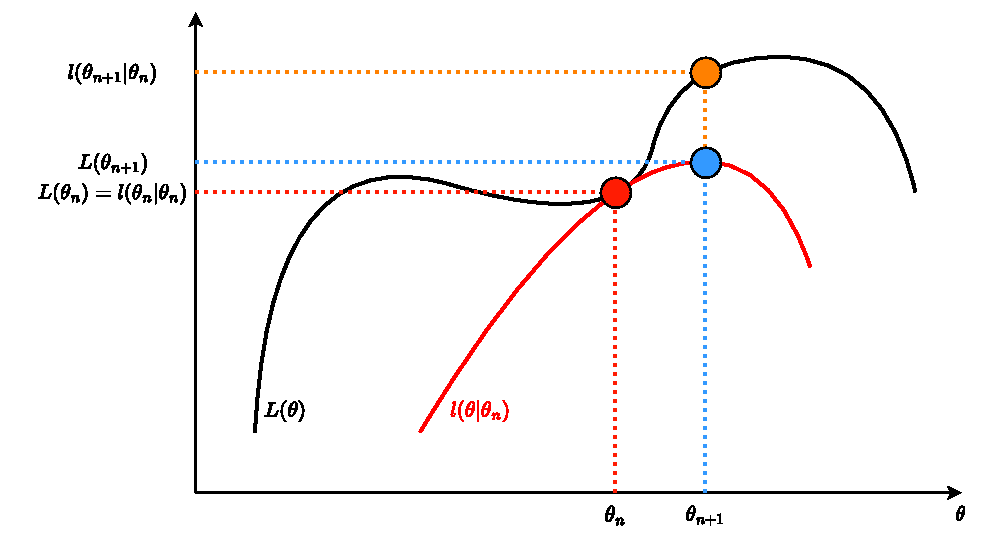
\includegraphics[height=180px]{Immagini/Modello base/Grafico verosimiglianza}
	\caption[Confronto tra la vera funzione di verosimiglianza $L(\theta)$ e la sua approssimazione in $\theta_n$.]{confronto tra la vera funzione di verosimiglianza $L(\theta)$ e la sua approssimazione in un intorno di $\theta_n$. Da notare che lo stimatore $l(\theta |\theta_n)$ non sovrastima la funzione reale.}
	\label{grafico_verosimiglianza}
\end{figure}

\subsection{Derivazione del passo M}
Dopo aver stimato nel passo E l'approssimazione $l(\boldsymbol{\theta}|\boldsymbol{\theta}_n)$  della vera funzione di verosimiglianza $L(\boldsymbol{\theta})$, è necessario ottimizzarla per determinare $\boldsymbol{\theta}_{n+1}$. Nello specifico:
\begin{equation}
	\begin{split}
		\boldsymbol{\theta}_{n+1} & = \text{arg}\,\max\limits_{\boldsymbol{\theta}}\  l(\boldsymbol{\theta}|\boldsymbol{\theta}_n) \\
		& =  \text{arg}\,\max\limits_{\boldsymbol{\theta}}\left\{ \textcolor{orange}{L(\boldsymbol{\theta}_n)} + \sum_{\mathbf{z}}^{} P(\mathbf{z}|\mathbf{x},\boldsymbol{\theta}_n)\cdot\ln\frac{P(\mathbf{x}|\mathbf{z},\boldsymbol{\theta})\cdot P(\mathbf{z}|\boldsymbol{\theta})}{\textcolor{orange}{P(\mathbf{z}|\mathbf{x},\boldsymbol{\theta}_n)}\cdot\textcolor{orange}{P(\mathbf{x}|\boldsymbol{\theta}_n)}}\right\} \\
		& = \text{arg}\,\max\limits_{\boldsymbol{\theta}}\left\{\sum_{\mathbf{z}}^{} P(\mathbf{z}|\mathbf{x},\boldsymbol{\theta}_n)\cdot\ln\textcolor{blue}{ P(\mathbf{x}|\mathbf{z},\boldsymbol{\theta})\cdot P(\mathbf{z}|\boldsymbol{\theta})}\right\}\\
		& = \text{arg}\,\max\limits_{\boldsymbol{\theta}}\left\{\sum_{\mathbf{z}}^{}P(\mathbf{z}|\mathbf{x},\boldsymbol{\theta}_n)\cdot\ln \textcolor{blue}{P(\mathbf{x},\mathbf{z}|\boldsymbol{\theta})}\right\}\\
		& = \text{arg}\,\max\limits_{\boldsymbol{\theta}}\left\{\text{E}_{\mathbf{z}|\mathbf{x},\boldsymbol{\theta}_n}\ln P(\mathbf{x},\mathbf{z}|\boldsymbol{\theta})\right\}\\
		& = \text{arg}\,\max\limits_{\boldsymbol{\theta}}\ Q(\boldsymbol{\theta},\boldsymbol{\theta}_n).
	\end{split}
\label{eq_derivazione_step_M}
\end{equation}
I termini in arancione vengono rimossi poiché costanti rispetto a $\boldsymbol{\theta}$, quindi non influenzano la ricerca dell'ottimo, mentre a quelli blu viene applicato il teorema di Bayes. \par Attraverso la riscrittura di $l(\boldsymbol{\theta}|\boldsymbol{\theta}_n)$ in $Q(\boldsymbol{\theta},\boldsymbol{\theta}_n)$ mediante la derivazione \ref{eq_derivazione_step_M}, si può comprendere l'idea che sta alla base dell'algoritmo EM: la log-verosimiglianza viene iterativamente corretta tramite la stima corrente della densità di probabilità delle variabili latenti $\mathbf{z}$, un'approssimazione ottenuta nel passo E a partire dai dati osservati $\mathbf{x}$ e dalla stima corrente dei coefficienti $\boldsymbol{\theta}_n$.
